\section{L11-Convezione}
\subsection{Introduzione}
La \textbf{convezione} identifica il trasporto di energia associato al
moto macroscopico del sistema: è quindi un processo che si
verifica tra la superficie di un corpo ed un fluido in moto
relativo.\newline
Si può classificare in due tipologie:
\begin{itemize}
    \item \textbf{Convezione forzata}: il moto del fluido è imposto da un agente esterno (per es. un ventilatore);
    \item \textbf{Convezione naturale} (solo all'interno di un campo gravitazionale): il moto del fluido è causato dal processo di trasmissione del calore che causa spinte di galleggiamento (per via delle differenze di densità).
\end{itemize}
\subsubsection{Fluidodinamica}
Per poter determinare il valore di scambio termico $h$, dobbiamo capire come si muove un fluido attorno all'oggetto studiato (cioè attorno a una parete).\newline
\newline
La trasmissione del calore per convezione è \textbf{fortemente legata} alla dinamica del
fluido che lambisce la parete solida.
\begin{itemize}
    \item In molte situazioni il moto del fluido \textbf{non assume una soluzione analitica}
    (natura tridimensionale e non lineare);
    \item Per questa ragione l’approccio utilizzato è di tipo \textbf{sperimentale} con
    l’introduzione di una \textbf{legge fenomenologica}
    \[
        \frac{\delta \rho}{\delta t} + \nabla \cdot (\rho \vec{u}) = 0
    \]
    \[
        \frac{\delta \rho \vec{u}}{\delta t} + \nabla \cdot  (\rho \vec{u} \vec{u}) = - \nabla P + \nabla \cdot \left[\mu \left(\nabla \vec{u} + \nabla \vec{u}^T\right)\right]
    \]
    per via di $ \nabla \cdot \rho \vec{u} \vec{u}$ si ha una non linearità. Queste espressioni sono molto difficili da anlizzare, e perciò, a parte per pochissimi casi particolari, non si riesce ad avere una soluzione analitica, cioè queste equazioni spesso non si riescono a risolvere.
\end{itemize}
\subsubsection{Legge di Newton}
\[
    J = h (T_p - T_f)
\]
dove \newline
$h =$ coefficiente di scambio termico convettivo $[W/m^2 K]$\newline
$T_p =$ temperatura della parete solida $[K]$\newline
$T_f =$ temperatura del fluido $[K]$\newline
\newline
Tutta la complessità delle equazioni del paragrafo precedente è concentrata all'interno del parametro $h$ (coefficiente di scambio termico convettivo).\newline
Il coefficiente di scambio convettivo (o conduttanza convettiva) dipende da:
\begin{itemize}
    \item proprietà fisiche del fluido;
    \item dinamica del flusso;
    \item geometria della superficie della parete.
\end{itemize}
\ \newline
\textbf{Valori generici del coefficiente convettivo}:\newline
\[
    \begin{matrix}
        \text{gas stagnante}\; & 5-50 \; [W/m^2K]\\
        \text{acqua stagnante}\;& 100 \; [W/m^2K]\\
        \\
        \text{gas in moto}\; & 15-1000 \; [W/m^2K]\\
        \text{olio minerale}\; & 50-3000\; [W/m^2K]\\
        \text{acqua in moto}\; &200-10000\; [W/m^2K]\\
        \\
        \text{acqua in ebollizione o condensazione}\; &1000-100000\; [W/m^2K]\\
        \text{metalli liquidi}\; &10000-100000\; [W/m^2K]\\
    \end{matrix}
\]
\subsubsection{Temperatura del fluido}
Non è facile attribuire un ben preciso valore per $T_f$ nella legge di Newton, in
quanto il fluido è generalmente sede di un gradiente termico e la sua temperatura
varia da punto a punto.
\begin{itemize}
    \item L’esperienza mostra che il gradiente termico è particolarmente accentuato
    nello strato di fluido direttamente a contatto con la parete (detto \textbf{strato limite
    termico})
    \item I criteri di scelta o definizione di $T_f$ risulteranno in generale quelli della
    \textbf{semplicità} di determinazione e di \textbf{significatività}
    \item Le definizioni di $T_f$ saranno diverse per ogni configurazione geometrica
    \item Nel caso di un fluido che lambisce esternamente un corpo solido (\textbf{convezione
    esterna}), si utilizza come temperatura $T_f$ la cosiddetta \textbf{temperatura
    asintotica} $T_\infty$ (lontano dalla parete, dove la temperatura è praticamente costante), ovvero la temperatura del fluido misurata in un punto in cui è
    praticamente nulla l’influenza della parete del solido
    \item Nel caso invece di un fluido che scorre all’interno di un condotto (\textbf{convezione
    interna}) si possono adottare diverse soluzioni anche se è maggiormente
    diffuso l’utilizzo della \textbf{temperatura di miscelamento adiabatico}, definita
    come:
    \[
        T_m = \frac{\int_{S}\rho c_P T w dS}{\int_{S}\rho c_P w dS}
    \]
    con $\rho$ massa volumica del fluido $[kg/m^3]$, $c_P$ calore specifico del fluido $[j/kgK]$, $w$ velocità del fluido $[m/s]$, $S$ sezione del condotto $[m^2]$.
\end{itemize}
\subsubsection{Il moto dei fluidi: esempio della lastra piana}
Si consideri il moto di un fluido su una lastra piana non in movimento.
\begin{center}
    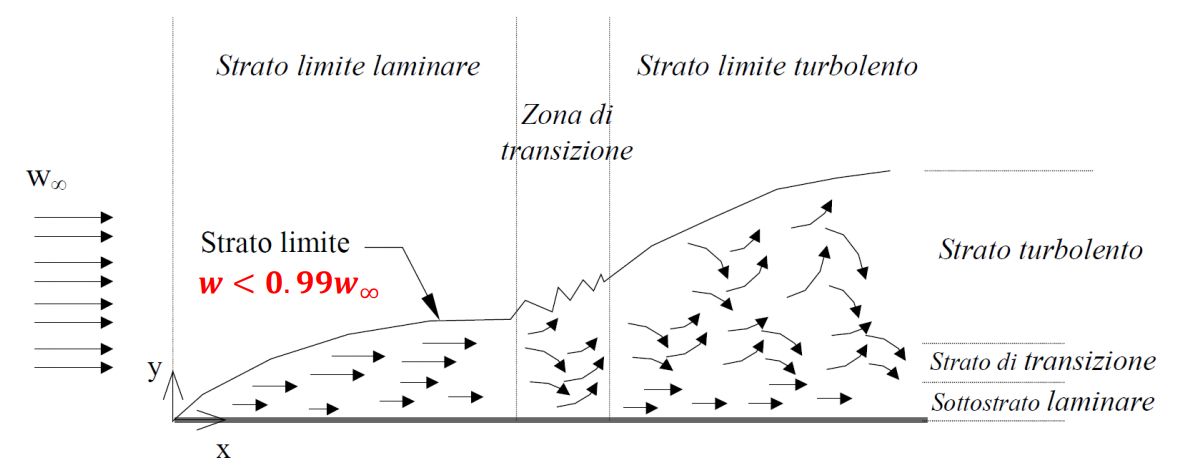
\includegraphics[height=3cm]{../L11/img1.PNG}
\end{center}
Video dimostrativo: \url{https://www.youtube.com/watch?v=wXsl4eyupUY}\newline
\newline
\begin{itemize}
    \item Negli strati adiacenti allo strato aderente alla lastra le particelle del fluido per
    effetto della viscosità tenderanno progressivamente a raggiungere la velocità
    indisturbata $w_{\infty}$. In questi strati sono influenti le sollecitazioni di taglio viscose
    (attrito) e la regione in cui la velocità è inferiore alla velocità indisturbata è
    detta zona di \textbf{strato limite} ($w < 0,99 w_{\infty}$).
    \item Un moto è denominato \textbf{laminare} se ordinato (o stabile) ovvero se i singoli filetti fluidi si muovono tutti parallelamente tra loro.
    \item Un moto è denominato \textbf{turbolento} se caratterizzato da variazioni di velocità e moto disordinato (o instabile) con componenti di velocità trasversali (vortici).
    \item In generale la \textbf{transizione} tra moto laminare e turbolento non avviene bruscamente ma esiste una regione nella quale il moto fluttua tra laminare e turbolento prima di diventare completamente instabile e perciò turbolento.
    \item La dimostrazione sperimentale dell'esistenza di diversi \textbf{regimi di moto} è dovuta a \textbf{Osborne Reynolds} che nel 1880 eseguì una serie di esperienze al fine di comprendere come si potesse descrivere il movimento di un fluido.
\end{itemize}
\subsection{Convezione forzata}
\subsubsection{L'analisi dimensionale}